
\section{Freedom and \iconfluence}
\label{sec:bcc-theory}

With a system model in hand, we now address the question: under what
conditions does a transaction require synchronous coordination? The
answer will depend on the set of operations the database may be
expected to perform as well as the integrity constraints that the
database is required to maintain.

We begin by introducing the concept of invariant confluence
(hereafter, \iconfluence)~\cite{obs-confluence}. Applied in a
transactional context, the \iconfluence property ensures that if the
effects of two series of separate transactions ($S_i$, $S_j$) that
operate independently on the same copy of valid database state are
valid ($I(S_i(D))$, $I(S_j(D))$ hold), their effects can safely be
combined to produce a valid database state ($I(S_i(D) \sqcup S_j(D))$
holds). \iconfluence will form the formal basis of a relationship
between \cfreedom and a set of invariants.

We first define a valid sequence of transformations, with represents
the results of applying a set of transactions to database state such
that each intermediate state is valid:

\begin{definition}[Valid Sequence]
Given invariant $I$ and $\{t_{i1}, \dots, t_{in}\} \in T$, $S_i(D) =
t_{in}(\dots t_{i1}(D))$ is an $I$-valid sequence of transactions in
$T$ if each $t_{ik}(\dots t_{i1}(D))$ is valid under $I$.
\end{definition}

Using the concept of valid sequences, we can formalize the
\iconfluence property, which ensures that the set of valid sequences
with a common ancestor are valid under merge:

\begin{definition}[\iconfluence]
Given invariant $I$, transactions $T$ are $I$-confluent if, for all
$I$-valid sequences $S_1(D_0)$, $S_2(D_0)$ of transactions in $T$,
$I(S_1(D_0) \sqcup S_2(D_0))$ is $I$-valid.
\end{definition}

Figure~\ref{fig:iconfluence} depicts an \iconfluent execution using
two valid sequences each starting from the initial database state
$D_0$. This execution model will be familiar to users of fork-join
programming models~\cite{hewitt-forkjoin} (e.g., version control
systems like Git and Subversion). \iconfluence allows users to ``check
out'' a known good copy of database state ($I(D)$) and perform
modifications to the state in isolation---as long as these
modifications are ``safe'' ($I(S_i(D))$ is true). Under \iconfluent
operations, any concurrent modifications to database state can be
safely ``merged'' to provide a valid database state ($I(S_1(D) \cup
S_2(D))$ is true). As we have alluded, \iconfluence depends on the
semantics of updates: an experienced programmer can likely think of
several operations and invariants that are not \iconfluent as well as
many that are. For example, if $I=\textit{no bank account has negative
  balance}$, then $T=\{\textit{increment user A's balance by 100,
  increment user A's balance by 50}\}$ is \iconfluent, as is
$T\cup\{$\textit{audit the database and store the sum of user balances
  in the \textrm{audit} table}$\}$ but not $T\cup\{$\textit{decrement
  user A's balance by 200}$\}$. We defer a full discussion of the
space of operations until Section~\ref{sec:bcc-practice}.

\begin{figure}
\begin{center}
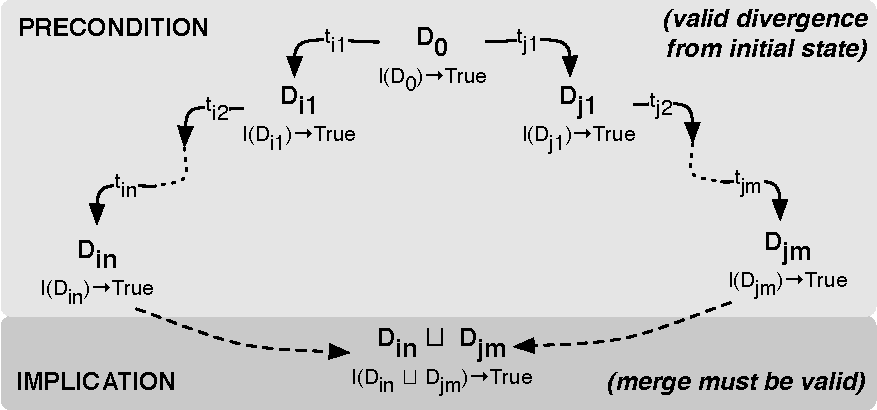
\includegraphics[width=\columnwidth]{figs/icommute.pdf}\vspace{-1em}
\end{center}
\caption{The \iconfluence property illustrated via a diamond
  diagram. If a set of transactions $T$ is \iconfluent, then all
  database states ($D_{in}$, $D_{jm}$) produced by $I$-valid sequences
  in $T$ starting from the initial database state ($D_0$) must be
  mergeable ($\sqcup$) into an $I$-valid database state.}
\label{fig:iconfluence}
\end{figure}

\miniheadnostop{A note on \iconfluence} Our notion of \iconfluence
directly incorporates a user's application-level invariants as part of
transaction execution. We discuss specific trade-offs in
Section~\ref{sec:relatedwork}, but we note that this definition is
more general than related concepts like state-based
commutativity~\cite{weihl-thesis} or traditional
confluence~\cite{calm,termrewriting}. For example, in Lamport's
example from Section~\ref{sec:motivation}, the outcome of audit
transactions is not commutative or confluent with respect to deposit
transactions, but audit transactions and deposit transactions are
indeed confluent with respect to the invariant that the database does
not contain negative account balances. The use of invariants instead
of states will allow us to specify a \textit{necessary} and sufficient
condition (instead of simply a sufficient condition) for coordination
during execution.

\iconfluence is particularly useful because it is deeply connected to
coordination-free execution:

\begin{theorem}
\label{theorem:necessary}
An always valid system can guarantee an application with transactions
$T$ and invariants $I$ with \cfreedom, transactional availability,
convergence if and only if $T$ is $I$-confluent.
\end{theorem}

Theorem~\ref{theorem:necessary} establishes \iconfluence as a
necessary and sufficient condition for coordination-free
execution---the first such condition we are aware of. The proof of
this theorem is a reformulation of classic partitioning
arguments~\cite{gilbert-cap}. Informally, if \iconfluence holds, each
replica can simply check each transaction's modifications locally and
replicas can simply merge independent modifications to guarantee
convergence. For the converse, we construct a scenario under which a
replica cannot determine whether or not a non-\iconfluent update
should succeed without contacting another replica.

\begin{proof}
($\Leftarrow$) We begin with the simpler proof, which is by
  construction. Assume an invariant $I$ and set of transactions $T$
  are $I$-confluent. Consider a system in which, for each transaction
  that each database replica receives, it executes the transaction
  against a copy of its current state and checks whether or not the
  resulting state is valid under $I$ or not. If the resulting state is
  valid, the replica commits the transaction. If not, the replica
  aborts the transaction. Replicas exchange copies of their local
  states and merge them. No individual replica will contain an invalid
  modification, and, because $T$ is $I$-confluent, the merge of any
  two valid replica states (i.e., valid sequences, as constructed
  above) is valid; therefore, the converged database state will be
  valid. Transactional availability, convergence, and validity are all
  maintained via coordination-free execution.

($\Rightarrow$) Assume a system $S$ exists that can guarantee always
  valid operation for a set of transactions $T$ with \cfreedom,
  transactional availability, and convergence, but $T$ is not
  $I$-confluent. Then there exists valid sequences $T_1,T_2$ in $T$
  such that $I(T_1(D_0)) \wedge I(T_2(D_0))$ is true but $I(T_1(D_0)
  \sqcup I(T_2(D_0))$ is false. We now construct two executions of $S$
  to produce a contradiction. Consider an execution $\alpha_1$ in
  which one replica $R_1$ executes the transactions from $T_1$ and a
  second execution $\alpha_2$ in which a second replica $R_2$ executes
  the transactions from $T_2$ and each replica initially contains the
  initial state $D_0$. Without synchronous communication, a third
  execution $\alpha_3$ containing the operations in both $\alpha_1$
  and $\alpha_2$---that is, $T_1$ is submitted to $R_1$ and $T_2$ is
  submitted to $R_2$---is, from the perspective of $R_1$,
  indistinguishable from $\alpha_1$, and, from the perspective of
  $R_2$, indistinguishable from $\alpha_2$. To preserve availability,
  in $\alpha_1$ and $\alpha_2$, $R_1$ and $R_2$ cannot choose to abort
  any of $T_1$ or $T_2$, yet, in $\alpha_3$, if $R_1$ and $R_2$ each
  commit their respective sequences, the merged state will be
  invalid. Therefore, $R_1$ and $R_2$ cannot simultaneously maintain
  valid state, \cfreedom, transactional availability, or convergence,
  as desired.
\end{proof}

Formalism aside, \iconfluence captures a simple rule; informally:
\textbf{Coordination is only required when a transaction's actions
  cannot be reconciled with concurrent actions.}  Alternatively (and
much less formally): \textbf{In a coordination-free system, any two
  valid database states must be mergeable into a valid database
  state.}

\minihead{Revisiting Payroll} Given \iconfluence, we can revisit our
payroll example. As we showed by counterexample, uniqueness of
arbitrary values is not \iconfluent: $\{$Stan:5$\}$ and $\{$Mary:5$\}$
are both valid states that can be reached by valid sequences (starting
at $\{\}$) but their merge---$\{$Stan:5, Mary:5$\}$ is not
valid. Therefore, insertion of arbitrary values is not $I$-confluent
for $I=\{$unique IDs$\}$. However, deletion of employees \textit{is}
$I$-confluent: removing items from a bag of unique values cannot
introduce duplicates. We can repeat the same exercise for foreign key
constraints: inserting new records with valid department IDs cannot in
fact introduce merge conflicts. The salary constraint is similarly
easily validated for simple insert statements. In the next section, we
will expand this analysis to a full SQL dialect.
